% 1. Replacez votre projet dans son contexte : enjeux scientifiques, enjeux sociétaux et/ou économiques (le cas échéant)
\begin{frame}{Contexte}

\begin{center}
  \begin{columns}
    \begin{column}{0.5\textwidth}
      Les  bases de données croissent rapidement

      \vspace{1em}
      Les algorithmes classiques sont parfois inefficaces
    \end{column}
    \begin{column}{0.5\textwidth}
      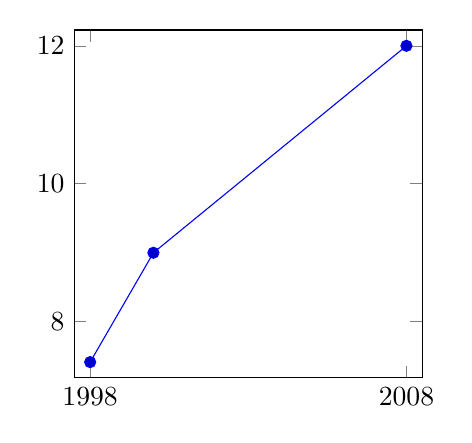
\begin{tikzpicture}
        \begin{axis}[
          width=6cm,height=6cm,
          x tick label style={
            /pgf/number format/1000 sep=},
          xtick = {1998,2008},
          enlargelimits=0.05,
          legend style={at={(0.5,0.1)},
          anchor=north,legend columns=-1},
        ]
        \addplot
          coordinates {(1998,7.414973347970818) (2000,9)
             (2008,12)};
        \end{axis}
      \end{tikzpicture}
    \end{column}
    \let\thefootnote\relax\footnotetext{$\log_{10}$ du nombre de pages indexées par Google}
    % https://googleblog.blogspot.com/2008/07/we-knew-web-was-big.html
  \end{columns}


  \pause
  Les \textbf{algorithmes quantiques} permettent de résoudre certains problèmes plus efficacement
  \end{center}
\end{frame}

\begin{frame}{Le besoin}
  Les machines quantiques sont en développement et resteront coûteuses financièrement
  $$\Downarrow$$
  Il y a un besoin d'outils de simulation et de vérification d'algorithmes quantiques
\end{frame}

\begin{frame}{Simulations}
  Les simulations sont très coûteuses en temps de calcul
  \begin{table}[]
    \begin{tabular}{l|l|l|l}
        \textit{Grover} & Classique & Quantique & Simulation    \\ \hline \rule{0pt}{2.6ex}
    Complexité & $N$       & $\sqrt N$ & {\color{red}$N \sqrt N$}
    \end{tabular}
    % https://arxiv.org/pdf/2005.04635
  \end{table}

  \vspace{1em}

  Elles nécessitent une \textbf{structure de données} adaptée
\end{frame}